%%%%%%%%%%%%%%%%%%%%%%%%%%%%%%%%%%%%%%%%%%%%%%%%%%%%%%%%%%%%%%%%%%%%%%%%%%%%%%%
% ARCHITECTURE DIAGRAMS - COMPLETE SIMULATION DESIGN
% 仿真架构图集 - Inbound, Outbound, 总体设计
%%%%%%%%%%%%%%%%%%%%%%%%%%%%%%%%%%%%%%%%%%%%%%%%%%%%%%%%%%%%%%%%%%%%%%%%%%%%%%%
% 包含3个TikZ架构图:
% 1. Inbound流程架构 (Figure 4.X-A)
% 2. Outbound流程架构 (Figure 4.X-B)
% 3. 总体仿真设计架构 (Figure 4.X-C) - Entity, Process, Constraint
%%%%%%%%%%%%%%%%%%%%%%%%%%%%%%%%%%%%%%%%%%%%%%%%%%%%%%%%%%%%%%%%%%%%%%%%%%%%%%%
% REQUIRES: \usepackage{tikz}
%           \usetikzlibrary{shapes,arrows,positioning,fit,backgrounds}
%%%%%%%%%%%%%%%%%%%%%%%%%%%%%%%%%%%%%%%%%%%%%%%%%%%%%%%%%%%%%%%%%%%%%%%%%%%%%%%

%=============================================================================
% DIAGRAM 1: INBOUND PROCESS ARCHITECTURE
% Inbound流程: Truck Arrival → Timeslot Allocation → Unloading → FTE Processing
%=============================================================================

\begin{figure}[h]
    \centering
    \scalebox{0.85}{  % 缩小到85%以适应页面
    \begin{tikzpicture}[
        node distance=1.5cm,  % 减小节点间距
        entity/.style={rectangle, draw, fill=blue!15, text width=2.3cm, text centered, rounded corners, minimum height=0.9cm, thick},
        process/.style={rectangle, draw, fill=green!20, text width=2.6cm, text centered, minimum height=0.95cm, thick},
        resource/.style={ellipse, draw, fill=orange!20, text width=2cm, text centered, minimum height=0.8cm, thick},
        constraint/.style={rectangle, draw, fill=red!15, text width=2.2cm, text centered, minimum height=0.75cm, dashed, thick},
        arrow/.style={->, >=stealth, thick},
        darrow/.style={->, >=stealth, thick, dashed, red}
    ]
        % ========== Main Flow (Left to Right) ==========
        % Stage 1: Arrival
        \node[entity] (arrival) {Truck Arrival\\(Poisson $\lambda_h$)};
        
        % Stage 2: Queue for Timeslot
        \node[process, right=2cm of arrival] (queue) {Queue for\\Reception Timeslot};
        
        % Stage 3: Unloading at Dock
        \node[process, right=2cm of queue] (unload) {Unloading\\(30 min)};
        
        % Stage 4: FTE Processing
        \node[process, right=2cm of unload] (processing) {FTE Process\\(24h limit)};
        
        % Stage 5: Completion
        \node[entity, right=2cm of processing] (complete) {Complete};
        
        % ========== Resources (Top) ==========
        \node[resource, above=1.8cm of queue] (timeslot) {Reception\\Timeslot\\Capacity};
        
        \node[resource, above=1.8cm of processing] (fte) {FTE Inbound\\Capacity\\(hourly)};
        
        % ========== Constraints (Bottom) ==========
        \node[constraint, below=1.5cm of queue] (timeslot_const) {Hourly\\Timeslot Limit\\(FG: 2, R\&P: 1)};
        
        \node[constraint, below=1.5cm of processing] (deadline) {24-hour\\Processing\\Deadline};
        
        % ========== Main Flow Arrows ==========
        \draw[arrow] (arrival) -- (queue);
        \draw[arrow] (queue) -- node[above, font=\small] {Allocated} (unload);
        \draw[arrow] (unload) -- node[above, font=\small] {Unloaded} (processing);
        \draw[arrow] (processing) -- (complete);
        
        % ========== Resource Constraint Arrows ==========
        \draw[darrow] (timeslot) -- node[right, font=\footnotesize] {Constrains} (queue);
        \draw[darrow] (fte) -- node[right, font=\footnotesize] {Constrains} (processing);
        
        % ========== Constraint Links ==========
        \draw[darrow] (timeslot_const) -- (queue);
        \draw[darrow] (deadline) -- (processing);
        
    \end{tikzpicture}
    }  % 结束scalebox
    \caption{Inbound process architecture: truck arrival, timeslot allocation, unloading, and FTE-constrained processing with 24-hour deadline.}
    \label{fig:inbound_architecture}
\end{figure}

%=============================================================================
% DIAGRAM 2: OUTBOUND PROCESS ARCHITECTURE
% Outbound流程: Order Pre-generation → Creation Time Trigger → FTE Processing → Pre-allocated Timeslot → Loading → Departure
%=============================================================================

\begin{figure}[h]
    \centering
    \scalebox{0.78}{  % 缩小以适应页面
    \begin{tikzpicture}[
        node distance=1.4cm,  % 减小节点间距
        entity/.style={rectangle, draw, fill=blue!15, text width=2.2cm, text centered, rounded corners, minimum height=0.85cm, thick},
        process/.style={rectangle, draw, fill=green!20, text width=2.4cm, text centered, minimum height=0.9cm, thick},
        resource/.style={ellipse, draw, fill=orange!20, text width=1.9cm, text centered, minimum height=0.75cm, thick},
        constraint/.style={rectangle, draw, fill=red!15, text width=2.1cm, text centered, minimum height=0.7cm, dashed, thick},
        decision/.style={diamond, draw, fill=purple!15, text width=1.5cm, text centered, minimum height=1.1cm, aspect=2, thick},
        pregen/.style={rectangle, draw, fill=cyan!15, text width=2.4cm, text centered, minimum height=0.85cm, thick, dashed},
        arrow/.style={->, >=stealth, thick},
        darrow/.style={->, >=stealth, thick, dashed, red},
        trigger/.style={->, >=stealth, thick, dotted, blue}
    ]
        % ========== Pre-generation Layer (Top) ==========
        \node[pregen] (pregen) {Order\\Pre-generation\\(12 months)};
        
        % ========== Main Flow (Left to Right) ==========
        % Stage 0: Creation Time Trigger
        \node[entity, below=1.5cm of pregen] (creation) {Creation Time\\Trigger};
        
        % Stage 1: FTE Processing
        \node[process, right=1.8cm of creation] (processing) {FTE Process\\(Prepare)};
        
        % Stage 2: Queue for Pre-allocated Timeslot
        \node[process, right=1.8cm of processing] (queue) {Wait for\\Pre-allocated\\Timeslot};
        
        % Stage 3: Loading at Dock
        \node[process, right=1.8cm of queue] (loading) {Loading\\(30 min)};
        
        % Stage 4: Departure Check
        \node[decision, right=1.8cm of loading] (check) {SLA\\Check};
        
        % Stage 5: Departure
        \node[entity, right=1.6cm of check] (depart) {Departure};
        
        % ========== Resources (Top) ==========
        \node[resource, above=1.6cm of processing] (fte) {FTE Outbound\\Capacity\\(hourly)};
        
        \node[resource, above=1.6cm of queue] (timeslot) {Pre-allocated\\Timeslot\\(at generation)};
        
        % ========== Constraints (Bottom) ==========
        \node[constraint, below=1.4cm of creation] (sim_window) {Simulation\\Window\\(720 hours)};
        
        \node[constraint, below=1.4cm of queue] (timeslot_const) {Hourly\\Timeslot Limit\\(FG: 1, R\&P: 4-6)};
        
        \node[constraint, below=1.4cm of check] (sla) {FG Departure\\Deadline\\(G2: same-day\\ROW: next-day)};
        
        % ========== Pre-generation Flow ==========
        \draw[trigger] (pregen) -- node[right, font=\footnotesize] {at creation time} (creation);
        
        % ========== Main Flow Arrows ==========
        \draw[arrow] (creation) -- node[above, font=\small] {Scheduled} (processing);
        \draw[arrow] (processing) -- node[above, font=\small] {Ready} (queue);
        \draw[arrow] (queue) -- node[above, font=\small] {Timeslot arrives} (loading);
        \draw[arrow] (loading) -- (check);
        \draw[arrow] (check) -- node[above, font=\small] {On-time} (depart);
        
        % ========== SLA Miss Path ==========
        \node[entity, below=2.3cm of check, fill=red!20] (delayed) {Delayed\\(SLA Miss)};
        \draw[arrow, red] (check) -- node[right, font=\footnotesize] {Late} (delayed);
        \draw[arrow] (delayed) -| (depart);
        
        % ========== Resource Constraint Arrows ==========
        \draw[darrow] (fte) -- node[right, font=\footnotesize] {Constrains} (processing);
        \draw[darrow] (timeslot) -- node[right, font=\footnotesize] {Allocated at\\generation} (queue);
        
        % ========== Constraint Links ==========
        \draw[darrow] (sim_window) -- (creation);
        \draw[darrow] (timeslot_const) -- (queue);
        \draw[darrow] (sla) -- (check);
        
    \end{tikzpicture}
    }  % 结束scalebox
    \caption{Outbound process architecture with pre-generation mechanism: orders are generated for 12 months with pre-allocated timeslots, but only those with creation time under 720 hours enter the 30-day simulation window. Each order is triggered at its creation time, then undergoes FTE-constrained processing, waits for its pre-allocated loading timeslot, completes loading, and undergoes SLA-based departure deadline check. G2 region requires same-day departure, ROW allows next-day.}
    \label{fig:outbound_architecture}
\end{figure}

%=============================================================================
% DIAGRAM 3: OVERALL SIMULATION DESIGN ARCHITECTURE
% 总体架构: Data Preparation → Simulation Execution → 核心组件
%=============================================================================

\begin{figure}[p]
    \centering
    \scalebox{0.72}{  % 缩小到72%以适应页面
    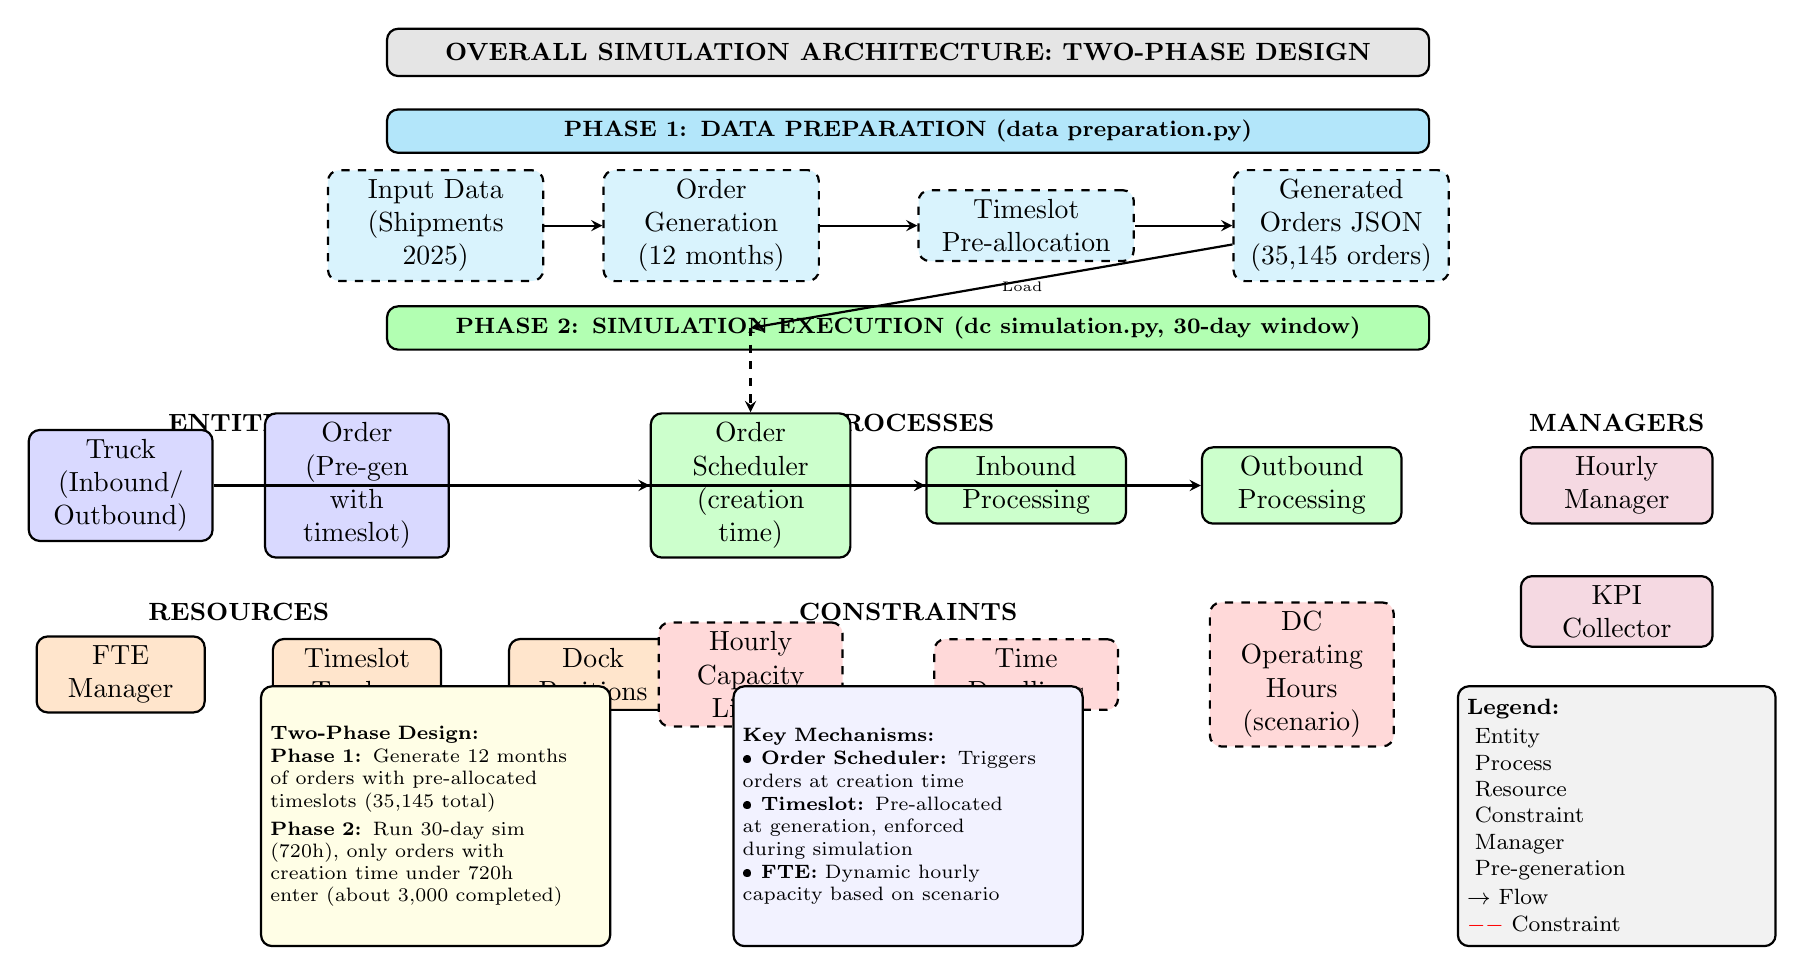
\begin{tikzpicture}[
        node distance=1.2cm,  % 减小节点间距
        box/.style={rectangle, draw, text width=2.1cm, text centered, rounded corners, minimum height=0.75cm, thick},
        entity/.style={box, fill=blue!15},
        process/.style={box, fill=green!20, text width=2.3cm},
        resource/.style={box, fill=orange!20, text width=1.9cm},
        constraint/.style={box, fill=red!15, dashed},
        manager/.style={box, fill=purple!15, text width=2.2cm},
        pregen/.style={box, fill=cyan!15, dashed, text width=2.5cm},
        arrow/.style={->, >=stealth, thick},
        darrow/.style={->, >=stealth, thick, dashed}
    ]
        % ========== TITLE BOXES (Top Layer) ==========
        \node[box, fill=gray!20, text width=13cm, minimum height=0.6cm, font=\bfseries\small] at (0, 7.5) 
            {OVERALL SIMULATION ARCHITECTURE: TWO-PHASE DESIGN};
        
        % ========== PHASE 1: DATA PREPARATION (Top Section) ==========
        \node[box, fill=cyan!30, text width=13cm, minimum height=0.55cm, font=\bfseries\footnotesize] at (0, 6.5) 
            {PHASE 1: DATA PREPARATION (data preparation.py)};
        
        \node[pregen] at (-6, 5.3) (input_data) {Input Data\\(Shipments\\2025)};
        \node[pregen] at (-2.5, 5.3) (generation) {Order\\Generation\\(12 months)};
        \node[pregen] at (1.5, 5.3) (timeslot_alloc) {Timeslot\\Pre-allocation};
        \node[pregen] at (5.5, 5.3) (output_json) {Generated\\Orders JSON\\(35,145 orders)};
        
        \draw[arrow] (input_data) -- (generation);
        \draw[arrow] (generation) -- (timeslot_alloc);
        \draw[arrow] (timeslot_alloc) -- (output_json);
        
        % ========== PHASE 2: SIMULATION EXECUTION (Main Section) ==========
        \node[box, fill=green!30, text width=13cm, minimum height=0.55cm, font=\bfseries\footnotesize] at (0, 4.0) 
            {PHASE 2: SIMULATION EXECUTION (dc simulation.py, 30-day window)};
        
        % ========== LAYER 1: ENTITY TYPES ==========
        \node[font=\bfseries\small] at (-8.5, 2.8) {ENTITIES};
        
        \node[entity] at (-10, 2) (truck) {Truck\\(Inbound/\\Outbound)};
        \node[entity] at (-7, 2) (order) {Order\\(Pre-gen\\with timeslot)};
        
        % ========== LAYER 2: PROCESS TYPES ==========
        \node[font=\bfseries\small] at (0, 2.8) {PROCESSES};
        
        \node[process] at (-2, 2) (scheduler) {Order\\Scheduler\\(creation time)};
        \node[process] at (1.5, 2) (inbound_p) {Inbound\\Processing};
        \node[process] at (5, 2) (outbound_p) {Outbound\\Processing};
        
        % ========== LAYER 3: RESOURCE TYPES ==========
        \node[font=\bfseries\small] at (-8.5, 0.4) {RESOURCES};
        
        \node[resource] at (-10, -0.4) (fte_res) {FTE\\Manager};
        \node[resource] at (-7, -0.4) (timeslot_res) {Timeslot\\Tracker};
        \node[resource] at (-4, -0.4) (dock_res) {Dock\\Positions};
        
        % ========== LAYER 4: CONSTRAINT TYPES ==========
        \node[font=\bfseries\small] at (0, 0.4) {CONSTRAINTS};
        
        \node[constraint] at (-2, -0.4) (hourly_c) {Hourly\\Capacity\\Limits};
        \node[constraint] at (1.5, -0.4) (time_c) {Time\\Deadlines};
        \node[constraint] at (5, -0.4) (operating_c) {DC\\Operating\\Hours\\(scenario)};
        
        % ========== LAYER 5: MANAGERS ==========
        \node[font=\bfseries\small] at (9, 2.8) {MANAGERS};
        
        \node[manager] at (9, 2) (hour_mgr) {Hourly\\Manager};
        \node[manager] at (9, 0.4) (kpi_mgr) {KPI\\Collector};
        
        % ========== CONNECTIONS ==========
        \draw[arrow] (output_json) -- node[right, font=\tiny] {Load} (-2, 4);
        \draw[arrow, dashed] (-2, 4) -- (scheduler);
        
        \draw[arrow] (order) -- (scheduler);
        \draw[arrow] (truck) -- (inbound_p);
        \draw[arrow] (scheduler) -- (outbound_p);
        
        % ========== LEGEND (Bottom Right) ==========
        \node[box, fill=gray!10, text width=3.8cm, minimum height=3.3cm, align=left, font=\footnotesize] at (9, -2.2) {
            \textbf{Legend:}\\[0.04cm]
            \textcolor{blue!70}{$\blacksquare$} Entity\\
            \textcolor{green!70}{$\blacksquare$} Process\\
            \textcolor{orange!70}{$\blacksquare$} Resource\\
            \textcolor{red!70}{$\blacksquare$} Constraint\\
            \textcolor{purple!70}{$\blacksquare$} Manager\\
            \textcolor{cyan!70}{$\blacksquare$} Pre-generation\\[0.04cm]
            $\rightarrow$ Flow\\
            \textcolor{red}{$- -$} Constraint
        };
        
        % ========== DETAILED NOTES (Bottom Left) ==========
        \node[box, fill=yellow!10, text width=4.2cm, minimum height=3.3cm, align=left, font=\scriptsize] at (-6, -2.2) {
            \textbf{Two-Phase Design:}\\[0.02cm]
            \textbf{Phase 1:} Generate 12 months\\of orders with pre-allocated\\timeslots (35,145 total)\\[0.08cm]
            \textbf{Phase 2:} Run 30-day sim\\(720h), only orders with\\creation time under 720h\\enter (about 3,000 completed)
        };
        
        \node[box, fill=blue!5, text width=4.2cm, minimum height=3.3cm, align=left, font=\scriptsize] at (0, -2.2) {
            \textbf{Key Mechanisms:}\\[0.02cm]
            • \textbf{Order Scheduler:} Triggers\\orders at creation time\\[0.02cm]
            • \textbf{Timeslot:} Pre-allocated\\at generation, enforced\\during simulation\\[0.02cm]
            • \textbf{FTE:} Dynamic hourly\\capacity based on scenario
        };
        
    \end{tikzpicture}
    }  % 结束scalebox
    \caption{Overall simulation design architecture showing two-phase approach: (1) Data Preparation phase generates 12 months of orders with pre-allocated timeslots using historical shipment data, producing 35,145 orders stored in JSON format; (2) Simulation Execution phase runs 30-day (720-hour) discrete event simulation, loading pre-generated orders but only processing those with creation time under 720h (approximately 3,000 orders completed). The architecture includes entity types (Truck, Order), process flows (Order Scheduler with creation time triggers, Inbound/Outbound processing), resource managers (FTE, Timeslot tracker, Dock), constraint mechanisms (Hourly capacity limits, Time deadlines, DC operating hours), and monitoring processes (Hourly manager, KPI collector).}
    \label{fig:simulation_architecture_overview}
\end{figure}

%%%%%%%%%%%%%%%%%%%%%%%%%%%%%%%%%%%%%%%%%%%%%%%%%%%%%%%%%%%%%%%%%%%%%%%%%%%%%%%
% USAGE NOTES
%%%%%%%%%%%%%%%%%%%%%%%%%%%%%%%%%%%%%%%%%%%%%%%%%%%%%%%%%%%%%%%%%%%%%%%%%%%%%%%
% :两阶段设计(Data Preparation + Simulation Execution)
%   - 展示12个月订单预生成 vs 30天仿真窗口的关系
%
% 第二步: 插入Inbound和Outbound架构图 (Figures 4.X-A, 4.X-B) 在各自章节
%   - 深入讲解具体流程
%   - 补充技术细节
%
% 三图对比:
% ─────────────────────────────────────────────────────────────────────────────
% │ 图名              │ 层次   │ 关注点                                  │ 适合章节    │
% ├──────────────────┼────────┼─────────────────────────────────────────┼─────────────┤
% │ Inbound Arch     │ 详细   │ 时间序列流程, 24h deadline              │ 4.3.X       │
% │ Outbound Arch    │ 详细   │ 订单预生成, creation_time调度, SLA检查   │ 4.3.X       │
% │ Overall Arch     │ 总览   │ 两阶段设计, 数据流, 12月→30天窗口映射    │ 4.3 总览    │
%
% 关键差异:
% ─────────────────────────────────────────────────────────────────────────────
% Inbound特点:
%   - 24小时处理deadline
%   - 单一流程:Arrival → Timeslot → Unload → Process
%   - Truck到达驱动(无预生成)
%
% Outbound特点:
%   - **订单预生成机制**:12个月订单在data_preparation.py中生成
%   - **creation_time调度**:订单按creation_time进入仿真(仅≤720h的订单被处理)
%   - **Timeslot预分配**:订单生成时已分配timeslot(不是运行时竞争)
%   - 两阶段流程:先Process后Loading(与Inbound相反)
%   - SLA检查(FG按region分类:G2 same-day, ROW next-day)
%
% Overall特点:
%   - **两阶段设计突出显示**:
%     Phase 1 - Data Preparation:生成全年订单(35,145个)
%     Phase 2 - Simulation Execution:运行30天窗口(~3,000个完成)
%   - 数据流追踪:Shipments 2025 → Order Generation → JSON → Simulation
%   - 窗口机制:12个月数据池 → creation_time过滤 → 30天仿真
%   - 全局视角:包含所有管理器(Hourly, KPI, Order Scheduler)
%   - 交互关系:实线=流程,虚线=约束│ 时间序列流程, 24h deadline│ 4.3.X       │
% │ Outbound Arch    │ 详细   │ 两阶段流程, SLA检查        │ 4.3.X       │
% │ Overall Arch     │ 总览   │ 组件类型, 交互关系         │ 4.3 总览    │
%
% 关键差异:
% ─────────────────────────────────────────────────────────────────────────────
% Inbound特点:
%   - 24小时处理deadline
%   - 单一流程:Arrival → Timeslot → Unload → Process
%
% Outbound特点:
%   - 两阶段流程:先Process后Loading(与Inbound相反)
%   - SLA检查(FG按region分类:G2 same-day, ROW next-day)
%   - 混合到达模式(75% scheduled + 25% random)
%
% Overall特点:
%   - 抽象层次:展示Entity/Process/Resource/Constraint分类
%   - 全局视角:包含所有管理器(Hourly, KPI)
%   - 交互关系:实线=流程,虚线=约束,点线=监控
%
%%%%%%%%%%%%%%%%%%%%%%%%%%%%%%%%%%%%%%%%%%%%%%%%%%%%%%%%%%%%%%%%%%%%%%%%%%%%%%%
% END OF ARCHITECTURE DIAGRAMS
%%%%%%%%%%%%%%%%%%%%%%%%%%%%%%%%%%%%%%%%%%%%%%%%%%%%%%%%%%%%%%%%%%%%%%%%%%%%%%%
